\subsection{METRIZABLE TOPOLOGICAL SPACES}

DEFINITION 3. A metric on a set X is said to be compatible with a topology C on X if the topology defined by this metric coincides with C. A topological space is said to be metrizable if there exists a metric on X compatible with the topology of X.

\pandocbounded{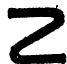
\includegraphics[keepaspectratio]{images/part001_d7e316f7.jpg}}

Two metrics on a set X which are both compatible with the same topology \(\mathfrak{C}\) can be inequivalent.

The subspace \(R_{+}^{*}\) of R provides an example of this. Both the uniformity induced by the additive uniformity of R and the uniformity induced by the multiplicative uniformity of \(R^{*}\) are metrizable and are compatible with the topology of \(R_{+}^{*}\) ; but they are not comparable.

We remark also that there can exist non-metrizable uniformities compatible with the topology of a metrizable topological space (Exercise 7).

We shall content ourselves here with necessary conditions for the metrizability of a topological space (for a necessary and sufficient condition, cf.~§ 4, Exercise 22). In the first place, a space cannot be metrizable unless it is completely regular (indeed we shall see, in § 4, no. 1, Proposition 2, that a metrizable space is necessarily ``normal'', which is a stronger condition). On the other hand, Theorem 1 shows that:

PROPOSITION 6. Every point of a metrizable space has a countable fundamental system of neighbourhoods.

More generally :

PROPOSITION 7. In a metrizable space, every closed set is the intersection of a countable family of open sets, and every open set is the union of a countable family of closed sets.

Let \(d\) be a metric compatible with the topology of a metrizable space \(\mathbf{X}\) . If \(\mathbf{A}\) is a closed subset of \(\mathbf{X}\) , it is the intersection of the open sets \(\mathrm{V}_{1/n}(\mathbf{A})\) {[}the set of all \(x\in\mathbf{X}\) such that \(d(x,\mathbf{A})<\mathbf{1}/n\) ; cf.~Proposition 2{]}. The second part of the proposition follows by taking complements.

Remarks. 1) These necessary conditions are not sufficient (cf.~Exercise 13). 2) There are spaces in which every point has a countable fundamental system of neighbourhoods but in which there exist closed sets which are not countable intersections of open sets (Exercise 15); such spaces are not metrizable.

Corollary 2 of Theorem 1, no. 4, shows that a countable product of metrizable topological spaces is metrizable. Also the sum X (Chapter I, § 2, no. 4) of an arbitrary family \((\mathbf{X}_t)_{t \in \mathbf{I}}\) of metrizable spaces is metrizable. For if \(d_t\) is a metric compatible with the topology of \(\mathbf{X}_t\) for each \(t \in \mathbf{I}\) , we may assume that \(d_t\) is bounded and that the diameter of \(\mathbf{X}_t\) is \(\leqslant t\) ; we can then define a distance \(d\) compatible with the topology of \(\mathbf{X}\) by putting \(d(x, y) = d_t(x, y)\) if \(x\) and \(y\) both belong to the same \(\mathbf{X}_t\) , and \(d(x, y) = t\) otherwise.

